\documentclass{standalone}
\usepackage{tikz}
\usetikzlibrary{patterns, positioning}
\usetikzlibrary{shapes.misc}
\usepackage[outline]{contour}
\contourlength{1.5pt} 


\begin{document}
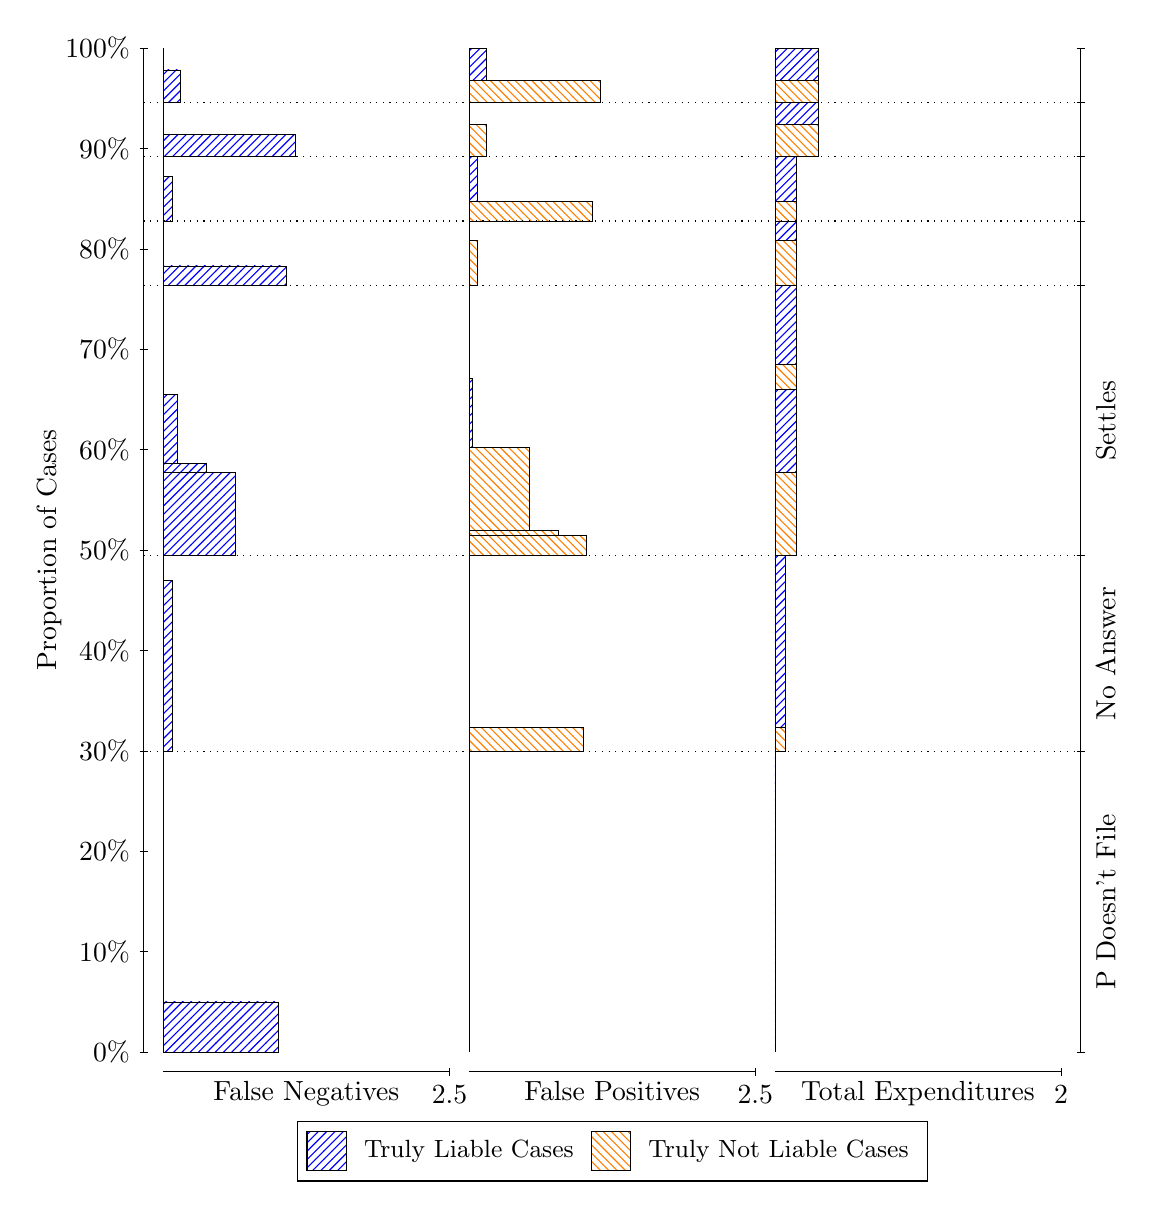
\begin{tikzpicture}
\draw[black, very thin] (1.5,1.75) -- (1.5,14.5);
\node[rotate=90, text=black, anchor=center] at (0.3, 8.125) {Proportion of Cases};
\draw[black, very thin] (1.45,1.75) -- (1.55,1.75);
\node[text=black, anchor=east] at (1.45, 1.75) {0\%};
\draw[black, very thin] (1.45,3.025) -- (1.55,3.025);
\node[text=black, anchor=east] at (1.45, 3.025) {10\%};
\draw[black, very thin] (1.45,4.3) -- (1.55,4.3);
\node[text=black, anchor=east] at (1.45, 4.3) {20\%};
\draw[black, very thin] (1.45,5.575) -- (1.55,5.575);
\node[text=black, anchor=east] at (1.45, 5.575) {30\%};
\draw[black, very thin] (1.45,6.85) -- (1.55,6.85);
\node[text=black, anchor=east] at (1.45, 6.85) {40\%};
\draw[black, very thin] (1.45,8.125) -- (1.55,8.125);
\node[text=black, anchor=east] at (1.45, 8.125) {50\%};
\draw[black, very thin] (1.45,9.4) -- (1.55,9.4);
\node[text=black, anchor=east] at (1.45, 9.4) {60\%};
\draw[black, very thin] (1.45,10.675) -- (1.55,10.675);
\node[text=black, anchor=east] at (1.45, 10.675) {70\%};
\draw[black, very thin] (1.45,11.95) -- (1.55,11.95);
\node[text=black, anchor=east] at (1.45, 11.95) {80\%};
\draw[black, very thin] (1.45,13.225) -- (1.55,13.225);
\node[text=black, anchor=east] at (1.45, 13.225) {90\%};
\draw[black, very thin] (1.45,14.5) -- (1.55,14.5);
\node[text=black, anchor=east] at (1.45, 14.5) {100\%};

\draw[black, very thin] (13.4,1.75) -- (13.4,14.5);
\draw[black, very thin] (13.35,1.75) -- (13.45,1.75);
\node[anchor=west] at (13.35, 1.75) {};
\draw[black, very thin] (13.35,5.5633) -- (13.45,5.5633);
\node[anchor=west] at (13.35, 5.5633) {};
\draw[black, very thin] (13.35,8.0532) -- (13.45,8.0532);
\node[anchor=west] at (13.35, 8.0532) {};
\draw[black, very thin] (13.35,11.483) -- (13.45,11.483);
\node[anchor=west] at (13.35, 11.483) {};
\draw[black, very thin] (13.35,12.303) -- (13.45,12.303);
\node[anchor=west] at (13.35, 12.303) {};
\draw[black, very thin] (13.35,13.123) -- (13.45,13.123);
\node[anchor=west] at (13.35, 13.123) {};
\draw[black, very thin] (13.35,13.812) -- (13.45,13.812);
\node[anchor=west] at (13.35, 13.812) {};
\draw[black, very thin] (13.35,14.5) -- (13.45,14.5);
\node[anchor=west] at (13.35, 14.5) {};

\draw[black, very thin, pattern color=blue, pattern=north east lines] (1.75,1.75) rectangle (3.2033,2.3857);
\draw[black, very thin, pattern color=orange, pattern=north west lines] (1.75,2.3857) rectangle (1.75,5.5633);
\draw[black, very thin, pattern color=blue, pattern=north east lines] (1.75,5.5633) rectangle (1.859,7.7423);
\draw[black, very thin, pattern color=orange, pattern=north west lines] (1.75,7.7423) rectangle (1.75,8.0532);
\draw[black, very thin, pattern color=blue, pattern=north east lines] (1.75,8.0532) rectangle (2.6583,9.1068);
\draw[black, very thin, pattern color=blue, pattern=north east lines] (1.75,9.1068) rectangle (2.295,9.2275);
\draw[black, very thin, pattern color=blue, pattern=north east lines] (1.75,9.2275) rectangle (1.9317,10.105);
\draw[black, very thin, pattern color=orange, pattern=north west lines] (1.75,10.105) rectangle (1.75,11.483);
\draw[black, very thin, pattern color=blue, pattern=north east lines] (1.75,11.483) rectangle (3.3123,11.732);
\draw[black, very thin, pattern color=orange, pattern=north west lines] (1.75,11.732) rectangle (1.75,12.303);
\draw[black, very thin, pattern color=blue, pattern=north east lines] (1.75,12.303) rectangle (1.859,12.874);
\draw[black, very thin, pattern color=orange, pattern=north west lines] (1.75,12.874) rectangle (1.75,13.123);
\draw[black, very thin, pattern color=blue, pattern=north east lines] (1.75,13.123) rectangle (3.4213,13.403);
\draw[black, very thin, pattern color=orange, pattern=north west lines] (1.75,13.403) rectangle (1.75,13.812);
\draw[black, very thin, pattern color=blue, pattern=north east lines] (1.75,13.812) rectangle (1.968,14.221);
\draw[black, very thin, pattern color=orange, pattern=north west lines] (1.75,14.221) rectangle (1.75,14.5);
\draw[black, very thin, pattern color=orange, pattern=north west lines] (5.6333,1.75) rectangle (5.6333,4.9276);
\draw[black, very thin, pattern color=blue, pattern=north east lines] (5.6333,4.9276) rectangle (5.6333,5.5633);
\draw[black, very thin, pattern color=orange, pattern=north west lines] (5.6333,5.5633) rectangle (7.0867,5.8741);
\draw[black, very thin, pattern color=blue, pattern=north east lines] (5.6333,5.8741) rectangle (5.6333,8.0532);
\draw[black, very thin, pattern color=orange, pattern=north west lines] (5.6333,8.0532) rectangle (7.123,8.308);
\draw[black, very thin, pattern color=orange, pattern=north west lines] (5.6333,8.308) rectangle (6.7597,8.3774);
\draw[black, very thin, pattern color=orange, pattern=north west lines] (5.6333,8.3774) rectangle (6.3963,9.4311);
\draw[black, very thin, pattern color=blue, pattern=north east lines] (5.6333,9.4311) rectangle (5.6697,10.309);
\draw[black, very thin, pattern color=blue, pattern=north east lines] (5.6333,10.309) rectangle (5.6333,11.483);
\draw[black, very thin, pattern color=orange, pattern=north west lines] (5.6333,11.483) rectangle (5.7423,12.054);
\draw[black, very thin, pattern color=blue, pattern=north east lines] (5.6333,12.054) rectangle (5.6333,12.303);
\draw[black, very thin, pattern color=orange, pattern=north west lines] (5.6333,12.303) rectangle (7.1957,12.552);
\draw[black, very thin, pattern color=blue, pattern=north east lines] (5.6333,12.552) rectangle (5.7423,13.123);
\draw[black, very thin, pattern color=orange, pattern=north west lines] (5.6333,13.123) rectangle (5.8513,13.532);
\draw[black, very thin, pattern color=blue, pattern=north east lines] (5.6333,13.532) rectangle (5.6333,13.812);
\draw[black, very thin, pattern color=orange, pattern=north west lines] (5.6333,13.812) rectangle (7.3047,14.091);
\draw[black, very thin, pattern color=blue, pattern=north east lines] (5.6333,14.091) rectangle (5.8513,14.5);
\draw[black, very thin, pattern color=orange, pattern=north west lines] (9.5167,1.75) rectangle (9.5167,4.9276);
\draw[black, very thin, pattern color=blue, pattern=north east lines] (9.5167,4.9276) rectangle (9.5167,5.5633);
\draw[black, very thin, pattern color=orange, pattern=north west lines] (9.5167,5.5633) rectangle (9.6529,5.8741);
\draw[black, very thin, pattern color=blue, pattern=north east lines] (9.5167,5.8741) rectangle (9.6529,8.0532);
\draw[black, very thin, pattern color=orange, pattern=north west lines] (9.5167,8.0532) rectangle (9.7892,9.1068);
\draw[black, very thin, pattern color=blue, pattern=north east lines] (9.5167,9.1068) rectangle (9.7892,10.16);
\draw[black, very thin, pattern color=orange, pattern=north west lines] (9.5167,10.16) rectangle (9.7892,10.485);
\draw[black, very thin, pattern color=blue, pattern=north east lines] (9.5167,10.485) rectangle (9.7892,11.483);
\draw[black, very thin, pattern color=orange, pattern=north west lines] (9.5167,11.483) rectangle (9.7892,12.054);
\draw[black, very thin, pattern color=blue, pattern=north east lines] (9.5167,12.054) rectangle (9.7892,12.303);
\draw[black, very thin, pattern color=orange, pattern=north west lines] (9.5167,12.303) rectangle (9.7892,12.552);
\draw[black, very thin, pattern color=blue, pattern=north east lines] (9.5167,12.552) rectangle (9.7892,13.123);
\draw[black, very thin, pattern color=orange, pattern=north west lines] (9.5167,13.123) rectangle (10.062,13.532);
\draw[black, very thin, pattern color=blue, pattern=north east lines] (9.5167,13.532) rectangle (10.062,13.812);
\draw[black, very thin, pattern color=orange, pattern=north west lines] (9.5167,13.812) rectangle (10.062,14.091);
\draw[black, very thin, pattern color=blue, pattern=north east lines] (9.5167,14.091) rectangle (10.062,14.5);
\draw[black, dotted] (1.5,5.5633) -- (13.4,5.5633);
\draw[black, dotted] (1.5,8.0532) -- (13.4,8.0532);
\draw[black, dotted] (1.5,11.483) -- (13.4,11.483);
\draw[black, dotted] (1.5,12.303) -- (13.4,12.303);
\draw[black, dotted] (1.5,13.123) -- (13.4,13.123);
\draw[black, dotted] (1.5,13.812) -- (13.4,13.812);
\draw[black, very thin] (1.75,1.5) -- (5.3833,1.5);
\node[text=black, anchor=north] at (3.5667, 1.5) {False Negatives};
\draw[black, very thin] (5.3833,1.45) -- (5.3833,1.55);
\node[text=black, anchor=north] at (5.3833, 1.45) {2.5};

\draw[black, very thin] (5.6333,1.5) -- (9.2667,1.5);
\node[text=black, anchor=north] at (7.45, 1.5) {False Positives};
\draw[black, very thin] (9.2667,1.45) -- (9.2667,1.55);
\node[text=black, anchor=north] at (9.2667, 1.45) {2.5};

\draw[black, very thin] (9.5167,1.5) -- (13.15,1.5);
\node[text=black, anchor=north] at (11.333, 1.5) {Total Expenditures};
\draw[black, very thin] (13.15,1.45) -- (13.15,1.55);
\node[text=black, anchor=north] at (13.15, 1.45) {2};

\node[text=black, centered, rotate=90] at (13.72, 3.6566) {\contour{white}{P Doesn't File}};
\node[text=black, centered, rotate=90] at (13.72, 6.8082) {\contour{white}{No Answer}};
\node[text=black, centered, rotate=90] at (13.72, 9.768) {\contour{white}{Settles}};





\draw (7.449999999999999,1.5) node[draw=none] (baseCoordinate) {};
\begin{scope}[align=center]
        \matrix[scale=0.5, draw=black, below=0.5cm of baseCoordinate, nodes={draw}, column sep=0.1cm]{
            \node[rectangle, draw, minimum width=0.5cm, minimum height=0.5cm, pattern color=blue, pattern=north east lines] {}; &
            \node[draw=none, font=\small, text=black] (B) {Truly Liable Cases}; &
            \node[rectangle, draw, minimum width=0.5cm, minimum height=0.5cm, pattern color=orange, pattern=north west lines] {}; &
            \node[draw=none, font=\small, text=black] (B) {Truly Not Liable Cases}; \\
            };
\end{scope}

\end{tikzpicture}
\end{document}